% American Journal of Physics submission manuscript — REVTeX 4.2.
% Double-spaced single-column review copy. For the typeset two-column journal
% look, change "preprint" -> "reprint" and comment out \doublespacing.
\documentclass[aip,preprint,amsmath,amssymb,floatfix]{revtex4-2}

\usepackage{graphicx}
\usepackage{booktabs}
\usepackage{setspace}
\usepackage{hyperref}

\doublespacing

\begin{document}

\title{Locating all Lagrange points with a curvature-learning MemComputing machine}

\author{Dietmar Henrich}
\affiliation{Chair of Materials Science and Nanotechnology,
Technische Universit\"{a}t Dresden, 01062 Dresden, Germany}

\author{Massimiliano Di Ventra}
\affiliation{Department of Physics, University of California San Diego,
La Jolla, CA 92093, USA}

\begin{abstract}
The MemComputing paradigm solves a problem by mapping its solutions onto the
stable fixed points of a dynamical system that is augmented with memory degrees of
freedom. Applied mostly to combinatorial optimization, it transfers naturally to a
classic continuous problem: the five Lagrange points of the restricted three-body
problem. A damped gradient flow on the Jacobi effective potential settles onto its
minima---the triangular points $L_4,L_5$---but is repelled by the collinear saddles
$L_1,L_2,L_3$, whose transverse direction is unstable. We turn the saddles into
attractors by inverting the force along that direction, a single sign that must be
$+1$ in the saddle's unstable direction and $-1$ at the stable minima. We show that
\emph{no constant choice works}, so this sign is the load-bearing ingredient---and
we let a memory supply it. The memory accumulates a quasi-Newton (Broyden) estimate
of the local curvature from the sequence of gradient evaluations the machine
already performs, with \emph{no} analytic second derivative, and from it sets the
inversion. The resulting autonomous flow with memory locates all five Lagrange
points of every Sun--planet and planet--moon pair of the solar system, twenty-three
systems with mass ratios from $\mu\approx2\times10^{-9}$ to $0.1$. The construction
is an instructive, fully reproducible example in which a memory degree of freedom
performs a genuine computation---learning the curvature of a landscape---that no
static rule can replace.
\end{abstract}

\maketitle

%=============================================================================
\section{Introduction and scope}\label{sec:intro}
%=============================================================================

MemComputing is a non-von-Neumann paradigm in which a physical system exploits
\emph{time non-locality}---the ability of internal degrees of freedom to retain and
use information about their past---to solve a problem~\cite{diventra2022}. In a
Digital MemComputing Machine the solutions of the target problem are mapped onto the
stable fixed points of a continuous dynamical system, and trajectories launched
from generic initial conditions are guided to a solution in an augmented phase space
whose coordinates are the relaxed original variables \emph{plus} the memory degrees
of freedom~\cite{traversa2015,diventra2018}. The paradigm has been applied mostly to
combinatorial optimization~\cite{traversa2017}; here we use it for a classic
continuous problem of celestial mechanics, and in doing so isolate a clean example
of a memory variable doing genuine computational work.

The restricted three-body problem (RTBP)---two primaries on a circular orbit and a
massless test particle---and its five Lagrange equilibria are a cornerstone of
nonlinear dynamics and of mission design~\cite{szebehely1967,lagrange1772}. The
equilibria are the critical points of the Jacobi effective potential $\Omega$. A
dissipative gradient flow is the natural dynamical-system route to such points, but
it has a basic limitation: damping drives a flow only to \emph{minima} of $\Omega$.
Two of the five Lagrange points (the triangular $L_4,L_5$) are minima and are found
this way; the other three (the collinear $L_1,L_2,L_3$) are \emph{saddles}, and a
damped flow is pushed away from them along their unstable direction. Making a saddle
into an attractor requires inverting the force along that direction---turning the
unstable direction into a restoring one. This single sign is what the machine must
supply, and supplying it correctly is the whole problem: the sign depends on the
local curvature of $\Omega$, which is positive at the minima and negative along the
saddles' unstable direction.

Our central observation is that \emph{no constant sign works}: inverting always
breaks the minima, never inverting never captures the saddles. The sign must track
the local curvature, and we let a memory degree of freedom do so. Crucially, the
memory does not read the analytic curvature; it \emph{learns} it, accumulating a
quasi-Newton estimate of the Hessian from the very gradient evaluations the flow
already performs, exactly as a Broyden or BFGS iteration builds curvature
information from a history of gradients~\cite{broyden1965,nocedal2006}. The
resulting machine---a single autonomous flow whose force inversion is controlled by
a curvature-learning memory---locates all five Lagrange points of every two-body
pair in the solar system, twenty-three systems spanning eight orders of magnitude in
mass ratio, with no analytic second derivative anywhere in the dynamics. We list
every parameter, give the off-axis controls that prove the memory is load-bearing,
and discuss honestly what the approach does and does not buy.

%=============================================================================
\section{The restricted three-body problem}\label{sec:rtbp}
%=============================================================================

We use the co-rotating frame in normalized units: the two primaries are separated by
unit distance, the orbital angular velocity of the frame is $\omega=1$, and the mass
ratio is
\begin{equation}
  \mu = \frac{M_2}{M_1+M_2}\in(0,\tfrac12],
\end{equation}
placing $M_1$ at $(-\mu,0)$ and $M_2$ at $(1-\mu,0)$. We define the effective
potential
\begin{equation}
  \Omega(x,y)=\frac{x^2+y^2}{2}+\frac{1-\mu}{r_1}+\frac{\mu}{r_2},
  \label{eq:omega}
\end{equation}
with $r_1=\sqrt{(x+\mu)^2+y^2}$ and $r_2=\sqrt{(x-1+\mu)^2+y^2}$. This is the
negative of the Jacobi potential commonly written with overall minus signs; with the
convention~\eqref{eq:omega} the Lagrange points are the critical points of $\Omega$,
and---as we use below---the triangular points are its \emph{minima}. The gradient is
\begin{align}
  \partial_x\Omega &= x-\frac{(1-\mu)(x+\mu)}{r_1^3}-\frac{\mu(x-1+\mu)}{r_2^3},
  \label{eq:gx}\\
  \partial_y\Omega &= y-\frac{(1-\mu)\,y}{r_1^3}-\frac{\mu\,y}{r_2^3}.
  \label{eq:gy}
\end{align}
A Lagrange point is a relative equilibrium, so the condition reduces to
\begin{equation}
  \boxed{\;\nabla\Omega(x,y)=\mathbf 0\;}
  \label{eq:clause}
\end{equation}
with exactly five solutions: the collinear $L_1,L_2,L_3$ on the axis $y=0$ and the
triangular $L_{4,5}=(\tfrac12-\mu,\pm\tfrac{\sqrt3}{2})$~\cite{szebehely1967}.

The \emph{nature} of each critical point---which is what the machine must
contend with---is set by the Hessian of $\Omega$. Its transverse component is
\begin{equation}
  \Omega_{yy}=1-\frac{1-\mu}{r_1^3}+\frac{3(1-\mu)y^2}{r_1^5}
              -\frac{\mu}{r_2^3}+\frac{3\mu y^2}{r_2^5}.
  \label{eq:oyy}
\end{equation}
On the axis ($y=0$) this reduces to $1-(1-\mu)/r_1^3-\mu/r_2^3$, which is
\emph{negative} at all three collinear points; together with
$\Omega_{xx}=1+2(1-\mu)/r_1^3+2\mu/r_2^3>0$ and $\Omega_{xy}=0$ there, the collinear
points are \emph{saddles}, unstable in the transverse ($y$) direction. At the
triangular points one finds $\Omega_{xx}=\tfrac34$, $\Omega_{yy}=\tfrac94$, and
$\Omega_{xy}=\tfrac{3\sqrt3}{4}(1-2\mu)$, giving $\det\mathrm{Hess}\,\Omega=
\tfrac{27}{4}\mu(1-\mu)>0$ with positive trace: $L_4,L_5$ are \emph{minima} of
$\Omega$. The sign of $\Omega_{yy}$ thus distinguishes the two cases: it is negative
in the unstable direction of the collinear saddles and positive at the triangular
minima (Fig.~\ref{fig:landscape}). The machine's task is to read this sign
correctly---ultimately, to learn it---using only information generated along its own
trajectory.

\begin{figure*}[!t]
  \centering
  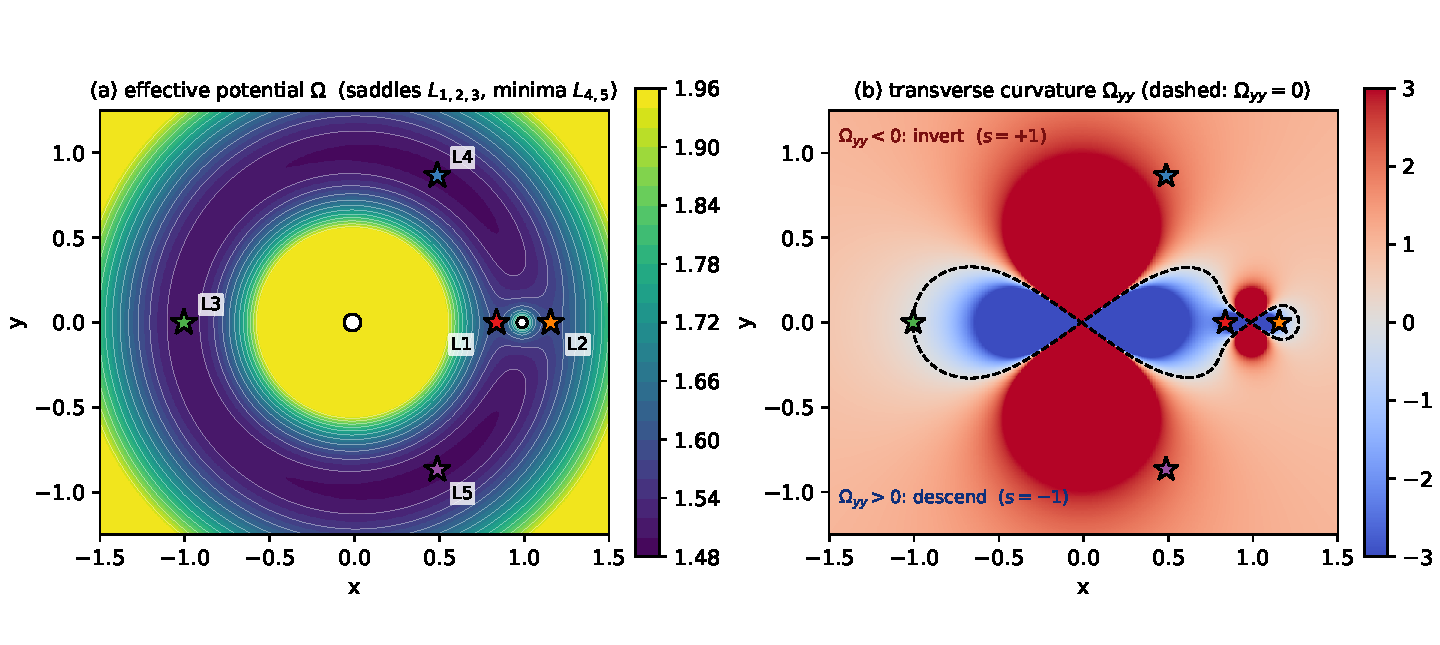
\includegraphics[width=0.96\textwidth]{fig_landscape.pdf}
  \caption{%
    The effective potential and its curvature for the Earth--Moon system
    ($\mu=0.0121$). \textbf{(a)} $\Omega(x,y)$, Eq.~\eqref{eq:omega}; the collinear
    $L_1,L_2,L_3$ are saddles and the triangular $L_4,L_5$ are minima; the large and
    small white dots are the primary and secondary. \textbf{(b)} the transverse
    curvature $\Omega_{yy}$, Eq.~\eqref{eq:oyy} (clipped at $\pm3$), with the contour
    $\Omega_{yy}=0$ dashed. Where $\Omega_{yy}<0$ (red) the machine inverts the
    transverse force ($s=+1$) to make the saddle attract; where $\Omega_{yy}>0$
    (blue) it descends normally ($s=-1$). The machine never reads this map; it learns
    the sign from its own gradient history.}
  \label{fig:landscape}
\end{figure*}

%=============================================================================
\section{Finding equilibria by landscape inversion}\label{sec:inversion}
%=============================================================================

Consider a damped flow that descends $\Omega$ in the rotating frame,
\begin{subequations}\label{eq:flow}
\begin{align}
  \ddot x &= 2\dot y-\partial_x\Omega-\gamma\dot x,\\
  \ddot y &= -2\dot x+s\,\partial_y\Omega-\gamma\dot y,
\end{align}
\end{subequations}
with constant viscosity $\gamma>0$ and an \emph{inversion gain} $s$ multiplying the
transverse force. With $s=-1$ the transverse force is the ordinary descent term
$-\partial_y\Omega$, which is restoring at a minimum; the flow then settles onto the
minima of $\Omega$, i.e.\ the triangular points $L_4,L_5$. At a collinear saddle,
however, the transverse direction has $\Omega_{yy}<0$: a small displacement $y>0$
gives $\partial_y\Omega<0$, so $-\partial_y\Omega>0$ pushes the particle
\emph{away} from the axis and the saddle repels. Setting $s=+1$ reverses this single
term into a restoring force, converting the saddle's unstable direction into a
stable one---the saddle becomes a minimum of the effective, inverted landscape and
an attractor of the flow.

The correct rule is therefore $s=-\operatorname{sign}(\Omega_{yy})$: invert
($s=+1$) where the transverse curvature is negative (the saddles), descend normally
($s=-1$) where it is positive (the minima). The key point is that this sign is
\emph{intrinsically position-dependent}, and \emph{no constant value of $s$ can
work}. We verify this directly. Seeding the flow off the symmetry axis---so that the
transverse direction is actually excited---around a collinear saddle ($L_1$) and
around a triangular minimum ($L_4$) of the Earth--Moon system, we record how many of
twelve seeds reach the target under each rule (Table~\ref{tab:noconstant}). A
constant $s=-1$ reaches the minimum from all seeds but \emph{never} the saddle; a
constant $s=+1$ reaches the saddle but \emph{breaks} the minimum, reaching it from
no seed. Only the curvature-adaptive sign captures both. The force inversion is thus
genuinely load-bearing---unlike the viscosity $\gamma$, which merely removes energy
and for which, we note, any constant value in a broad range suffices.

\begin{table}[ht]
\centering
\caption{No constant inversion works. Off-axis seeds (twelve each) around the
Earth--Moon collinear saddle $L_1$ and triangular minimum $L_4$; entries are the
number reaching the target under the raw dynamics~\eqref{eq:flow} (no refinement).
``adaptive'' is $s=-\operatorname{sign}(\Omega_{yy})$; ``memory'' is the
Hessian-free machine of Sec.~\ref{sec:memory}.}
\label{tab:noconstant}
\begin{tabular}{lcccc}
\toprule
seed region & $s\equiv-1$ & $s\equiv+1$ & adaptive & memory\\
\midrule
$L_1$ (collinear saddle) & $0/12$  & $12/12$ & $10/12$ & $11/12$\\
$L_4$ (triangular minimum) & $12/12$ & $0/12$  & $12/12$ & $12/12$\\
\bottomrule
\end{tabular}
\end{table}

%=============================================================================
\section{A memory that learns the curvature}\label{sec:memory}
%=============================================================================

The adaptive rule of Sec.~\ref{sec:inversion} requires the sign of $\Omega_{yy}$.
Reading it from the analytic Hessian~\eqref{eq:oyy} works, but it is unsatisfying:
the machine would be handed the very curvature information that distinguishes the
solutions. We instead let a memory degree of freedom \emph{learn} it. The flow
already evaluates the gradient $\mathbf g=\nabla\Omega$ at every step, and the
Jacobian of $\mathbf g$ is the Hessian. A memory matrix $B$ therefore accumulates a
\emph{quasi-Newton} estimate of the Hessian from successive gradient samples. With
$\Delta\mathbf p=\mathbf p_k-\mathbf p_{k-1}$ and
$\Delta\mathbf g=\mathbf g_k-\mathbf g_{k-1}$, the step from $B_k$ to $B_{k+1}$ adds a
Broyden secant assimilation~\cite{broyden1965,nocedal2006} and a slow relaxation
toward the identity,
\begin{equation}
  B_{k+1}=B_k
    +\frac{(\Delta\mathbf g-B_k\,\Delta\mathbf p)\,\Delta\mathbf p^{\mathsf T}}
          {\Delta\mathbf p^{\mathsf T}\Delta\mathbf p}
    +\lambda\,(\mathbf{1}-B_k)\,\Delta t ,
  \label{eq:broyden}
\end{equation}
applied only where $\lVert\Delta\mathbf p\rVert$ exceeds a small gate (otherwise
$B_{k+1}=B_k$); the right-hand side is then symmetrized to respect the symmetry of a
Hessian. The two added terms
are of different character. The first is the secant correction, which enforces
$B\,\Delta\mathbf p=\Delta\mathbf g$ along the current step: a full per-step
assimilation whose size is set by how wrong $B$ is and is \emph{independent} of
$\Delta t$ (Broyden is a discrete iteration, with no continuum limit as $\Delta t$
shrinks to zero). The second
is a genuine rate---a slow leak toward the identity. Because the curvature varies
across the landscape, this leak gives $B$ a finite memory horizon $\sim1/\lambda$, so
it tracks the \emph{local} curvature rather than a path-history average, and relaxing
toward $\mathbf{1}$ supplies a safe default ($B_{yy}=1$) where the step is too small to
measure. Equivalently, $B$ follows a continuous leak $\dot B=-\lambda(B-\mathbf{1})$
punctuated by discrete secant measurements---the structure of a continuous--discrete
(Kalman-type) estimator.
The estimated transverse curvature is the component $B_{yy}$, and the inversion gain
is a second memory variable $s\in[-1,1]$ that relaxes toward the learned sign,
\begin{equation}
  \dot s = \alpha\Bigl[-\tanh\!\Bigl(\tfrac{B_{yy}-\theta_s}{\varepsilon_c}\Bigr)-s
           \Bigr].
  \label{eq:sdot}
\end{equation}
The augmented phase space is thus $(x,y,\dot x,\dot y,\,s,\,B)$: the relaxed
mechanical variables plus the memory $(s,B)$. The full machine integrates
\eqref{eq:flow} with $\gamma$ constant, advancing $B$ by
\eqref{eq:broyden} and $s$ by \eqref{eq:sdot} at each step. No
analytic second derivative appears anywhere in the dynamics; $\Omega_{yy}$ is used
only, after the fact, to confirm that the learned $B_{yy}$ is correct.

Two features make the scheme work. First, it is \emph{predictive}. During the
off-axis approach to a saddle the trajectory samples gradients over a range of
positions, so $B$ accumulates a usable curvature estimate \emph{before} the
trajectory reaches the unstable region---it does not have to wait for the runaway to
develop. (A purely reactive detector, one that infers instability from the growth of
the motion, is outrun by the exponential instability of the saddle and fails; the
quasi-Newton accumulation is what makes the memory fast enough.) Second, the
threshold $\theta_s<0$ in~\eqref{eq:sdot} biases $s$ toward the safe descending
state $s=-1$, inverting only when the learned curvature is \emph{clearly} negative.
This protects the minima and the small-$\mu$ corotation ridge (where
$\lVert\nabla\Omega\rVert\approx0$ along $r=1$ and the curvature estimate hovers
near zero) while still inverting at genuine saddles, where $B_{yy}$ is strongly
negative. The bias is needed because the damped rotating frame is not symmetric
under sign reversal of $y$---the Coriolis term breaks it---so $L_4$ and $L_5$ have slightly
different basins; biasing toward the safe state treats both robustly.

Figure~\ref{fig:memory} shows the memory at work on two Earth--Moon trajectories. On
the approach to the collinear saddle $L_1$ the estimate $B_{yy}$ converges to a
negative value tracking the true $\Omega_{yy}$, and $s$ ramps from $-1$ to $+1$,
inverting the force and capturing the saddle. On the approach to the triangular
minimum $L_4$ the estimate is positive, $s$ stays at $-1$, and the flow descends
normally. The same memory, with no curvature supplied, discovers opposite signs in
the two cases.

\begin{figure*}[!t]
  \centering
  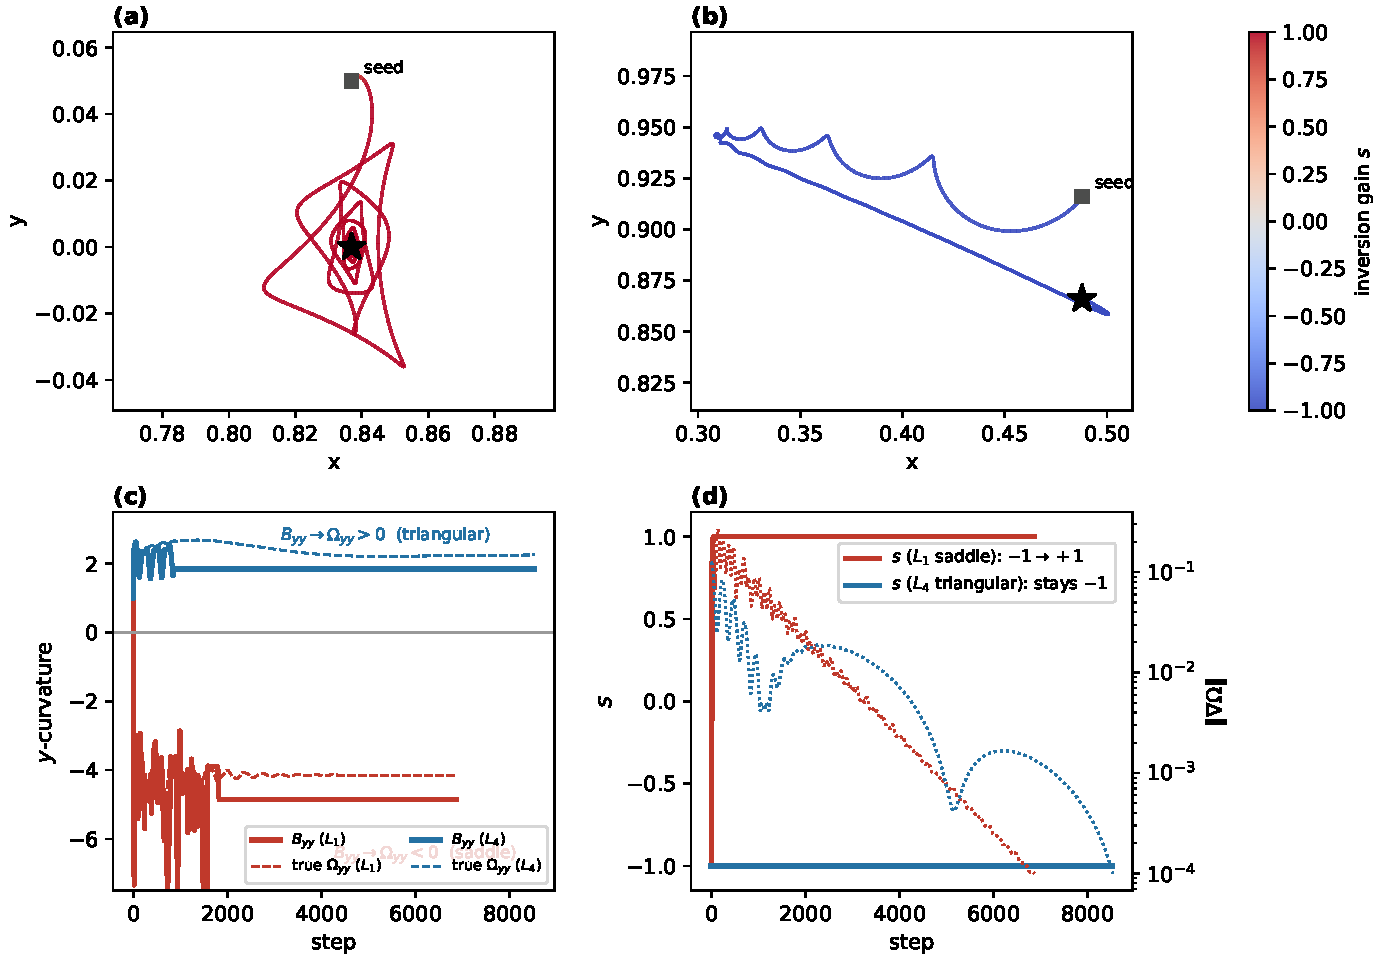
\includegraphics[width=0.98\textwidth]{fig_memory_curvature.pdf}
  \caption{%
    The memory learns the curvature. Two Earth--Moon trajectories of the same
    Hessian-free machine. \textbf{(a),(b)} phase-plane paths coloured by the
    inversion gain $s$: red ($s=+1$) on the approach to the collinear saddle
    $L_1$, blue ($s=-1$) on the approach to the triangular minimum $L_4$.
    \textbf{(c)} the quasi-Newton estimate $B_{yy}$ (solid) tracks the true
    $\Omega_{yy}$ (dashed) from gradient history alone---negative at the saddle,
    positive at the minimum. \textbf{(d)} the gain $s$ responds to what was learned:
    from $-1$ to $+1$ at the saddle, held at $-1$ at the minimum, while $\lVert\nabla\Omega
    \rVert$ (faint) decays to convergence.}
  \label{fig:memory}
\end{figure*}

%=============================================================================
\section{Numerical implementation and parameters}\label{sec:params}
%=============================================================================

Everything below is the procedure actually integrated in the accompanying
code~\cite{github2026}; the parameters are collected in Table~\ref{tab:params}.

\paragraph{Integration.}
The equations are advanced by explicit Euler with fixed step $\Delta t$; a guard
$\varepsilon=10^{-9}$ is added to $r_1,r_2$. The memory is initialized at
$B=\mathbf{1}$, $s=-1$ (the safe descending state), and the Broyden
update~\eqref{eq:broyden} is applied only when $\lVert\Delta\mathbf p\rVert$ exceeds
a small gate, so that near a fixed point---where $\Delta\mathbf p$ vanishes---the estimate
simply freezes. A trajectory stops when $\lVert\nabla\Omega\rVert<\theta$, when it
leaves the disk $\lVert\mathbf r\rVert>12$, or after $N_{\max}$ steps.

\paragraph{Seed grid.}
No solution coordinates are given to the integrator. Starting positions are
generated from the \emph{generic structure} of the RTBP only, using the Hill radius
$r_H=(\mu/3)^{1/3}$ and the secondary position $x_{\rm s}=1-\mu$:
(A) on-axis seeds $(x_{\rm s}\pm c\,r_H,0)$ for
$c\in\{0.5,0.7,1,1.4,2,3,5,8\}$, bracketing the collinear $L_1,L_2$;
(B) $L_3$ seeds near $x=-1$;
(C) equilateral seeds about $(\tfrac12,\pm\tfrac{\sqrt3}{2})$ for the triangular
points;
(D) a coarse off-axis fill for the broad large-$\mu$ basins.
Seeds inside the exclusion disks around either primary are discarded, leaving of
order seventy seeds per system. Even the equilateral seeds use the fixed
$(\tfrac12,\pm\tfrac{\sqrt3}{2})$ rather than the $\mu$-dependent solution; the
dynamics and the refinement below produce the exact positions.

\paragraph{Refinement and labelling.}
Each stopped trajectory is optionally polished by a few Newton iterations on
$\nabla\Omega=\mathbf 0$, accepted only if it reaches $\lVert\nabla\Omega\rVert
<10^{-9}$, otherwise the raw endpoint is kept. A converged point is identified with
the nearest analytic Lagrange position if within $0.05$ (polished) or $0.12$ (raw);
these analytic positions are used only for post-hoc identification, never by the
machine.

\begin{table}[ht]
\centering
\caption{Parameters used for all results, identical for every system.}
\label{tab:params}
\begin{tabular}{lll}
\toprule
Symbol & Meaning & Value\\
\midrule
$\gamma$ & viscosity (constant) & $0.3$\\
$\alpha$ & relaxation rate of the gain $s$ & $15$\\
$\varepsilon_c$ & curvature scale in Eq.~\eqref{eq:sdot} & $0.3$\\
$\lambda$ & Broyden leak toward $\mathbf{1}$ & $2.0$\\
$\theta_s$ & safe-state bias (invert if $B_{yy}<\theta_s$) & $-0.6$\\
$\lVert\Delta\mathbf p\rVert_{\min}$ & Broyden update gate & $10^{-4}$\\
$\Delta t$ & Euler time step & $0.01$\\
$\theta$ & convergence threshold $\lVert\nabla\Omega\rVert$ & $10^{-4}$\\
$N_{\max}$ & maximum steps & $1.2\times10^{5}$\\
$\varepsilon$ & singularity guard on $r_1,r_2$ & $10^{-9}$\\
accept & Newton refinement acceptance & $\lVert\nabla\Omega\rVert<10^{-9}$\\
\bottomrule
\end{tabular}
\end{table}

%=============================================================================
\section{Results}\label{sec:results}
%=============================================================================

The central result is that the curvature-learning machine, with the single
parameter set of Table~\ref{tab:params} and \emph{no analytic Hessian in its
dynamics}, discovers all five Lagrange points of every two-body system in the solar
system. Table~\ref{tab:systems} lists the twenty-three Sun--planet and planet--moon
pairs, with mass ratios spanning eight orders of magnitude, from Mars--Deimos
($\mu=2.3\times10^{-9}$) to Pluto--Charon ($\mu=0.11$). Every system returns $5/5$;
after the optional Newton polish the located positions agree with the analytic
Lagrange points to better than $10^{-9}$. Figure~\ref{fig:discovery} shows
trajectories of the machine reaching all five points of the Earth--Moon system from
the structural seed grid.

\begin{figure}[!t]
  \centering
  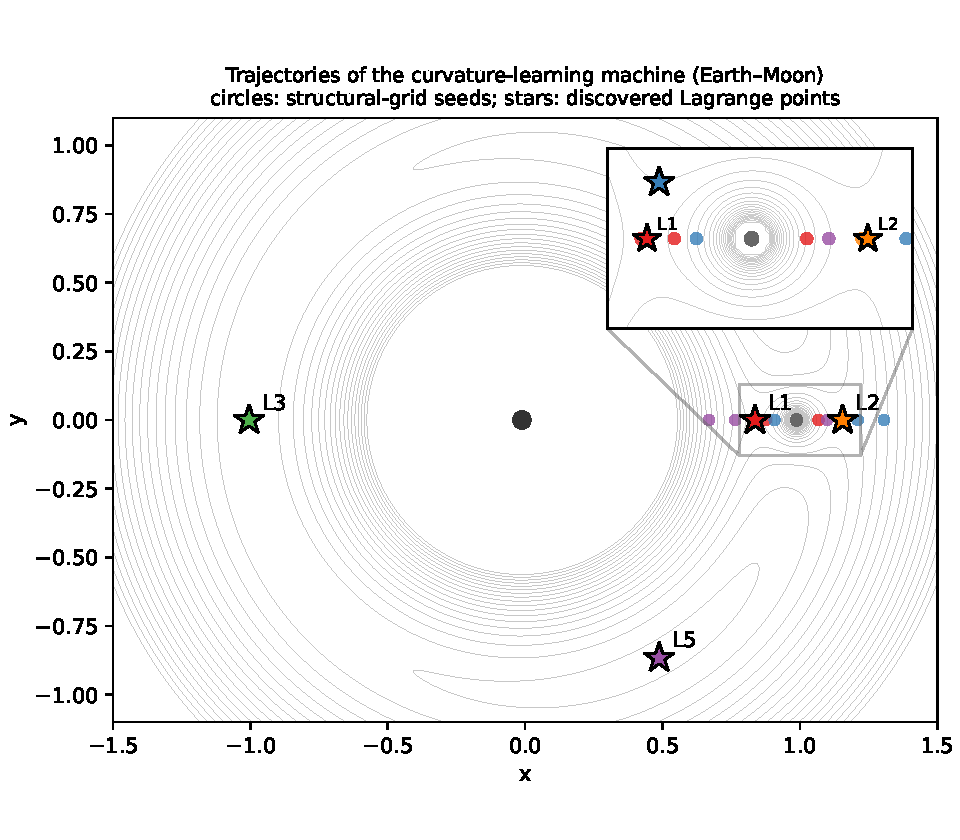
\includegraphics[width=0.99\columnwidth]{fig_discovery_qn.pdf}
  \caption{%
    Trajectories of the curvature-learning machine for the Earth--Moon system, each
    coloured by the Lagrange point it converges to (stars); circles mark the
    structural-grid seeds and grey curves are level sets of $\Omega$. The inset zooms
    the cramped $L_1/L_2$ region near the secondary. The machine receives no solution
    coordinates and no analytic curvature.}
  \label{fig:discovery}
\end{figure}

The off-axis controls of Table~\ref{tab:noconstant} establish the role of the
memory: it supplies a sign that no constant can. The smaller-$\mu$ systems are the
demanding ones---the triangular minima sit on the nearly flat corotation ridge---and
they are exactly where the safe-state bias $\theta_s$ matters; with it, the
Hessian-free machine matches the analytic-curvature machine across the whole range.
For reference, the identical machine driven by the analytic $\Omega_{yy}$ instead of
the learned $B_{yy}$ also returns $5/5$ on all twenty-three systems, so the
gradient-history estimate loses nothing.

\begin{table}[ht]
\centering
\caption{All five Lagrange points found for every solar-system pair by the
curvature-learning machine (no analytic Hessian in the dynamics), using the single
parameter set of Table~\ref{tab:params}. ``Stable'' refers to the linear stability
of $L_4,L_5$ (Routh, $\mu<0.03852$~\cite{routh1875}).}
\label{tab:systems}
\begin{tabular}{lccc}
\toprule
System & $\mu$ & Found & $L_4/L_5$ stable\\
\midrule
Mars--Deimos      & $2.3\times10^{-9}$ & $5/5$ & yes\\
Sun--Pluto        & $6.6\times10^{-9}$ & $5/5$ & yes\\
Mars--Phobos      & $1.7\times10^{-8}$ & $5/5$ & yes\\
Sun--Mercury      & $1.7\times10^{-7}$ & $5/5$ & yes\\
Saturn--Enceladus & $1.9\times10^{-7}$ & $5/5$ & yes\\
Sun--Mars         & $3.2\times10^{-7}$ & $5/5$ & yes\\
Sun--Venus        & $2.4\times10^{-6}$ & $5/5$ & yes\\
Sun--Earth        & $3.0\times10^{-6}$ & $5/5$ & yes\\
Saturn--Rhea      & $4.1\times10^{-6}$ & $5/5$ & yes\\
Jupiter--Europa   & $2.5\times10^{-5}$ & $5/5$ & yes\\
Uranus--Oberon    & $3.5\times10^{-5}$ & $5/5$ & yes\\
Uranus--Titania   & $4.1\times10^{-5}$ & $5/5$ & yes\\
Sun--Uranus       & $4.4\times10^{-5}$ & $5/5$ & yes\\
Jupiter--Io       & $4.7\times10^{-5}$ & $5/5$ & yes\\
Sun--Neptune      & $5.1\times10^{-5}$ & $5/5$ & yes\\
Jupiter--Callisto & $5.7\times10^{-5}$ & $5/5$ & yes\\
Jupiter--Ganymede & $7.8\times10^{-5}$ & $5/5$ & yes\\
Neptune--Triton   & $2.1\times10^{-4}$ & $5/5$ & yes\\
Saturn--Titan     & $2.4\times10^{-4}$ & $5/5$ & yes\\
Sun--Saturn       & $2.9\times10^{-4}$ & $5/5$ & yes\\
Sun--Jupiter      & $9.5\times10^{-4}$ & $5/5$ & yes\\
Earth--Moon       & $1.2\times10^{-2}$ & $5/5$ & yes\\
Pluto--Charon     & $1.1\times10^{-1}$ & $5/5$ & no\\
\bottomrule
\end{tabular}
\end{table}

%=============================================================================
\section{Why a memory, and what it does not do}\label{sec:discussion}
%=============================================================================

It is worth being precise about where the memory is, and is not, essential. The
viscosity $\gamma$ in~\eqref{eq:flow} removes energy and quenches the motion, but
this is a generic role: any constant $\gamma$ in a broad range damps the flow onto
the attractors equally well, and a time-varying or memory-controlled viscosity buys
nothing here. The inversion gain $s$ is different. As Table~\ref{tab:noconstant}
shows, the sign it carries cannot be constant---it must be $+1$ in the saddles'
unstable direction and $-1$ at the minima---so a degree of freedom that adapts it to
the local landscape is genuinely required. The memory is that degree of freedom, and
in its quasi-Newton form it does not merely store a number it was given: it
\emph{computes} the curvature, accumulating it from the history of gradient
evaluations the flow already performs. This is the sense in which the memory is the
active ingredient of the computation, and it is the clean lesson the example
teaches.

The construction has clear limits, which we state plainly. It does not compete with
classical root finders on speed: a Newton iteration converges in a handful of
evaluations once a bracket is known, far faster than integrating a trajectory, and
we retain an optional Newton polish for the final digits. The advantage is of a
different kind. The machine is \emph{global and prior-knowledge-free}: one autonomous
flow, one parameter set, locates all five equilibria of any system from a generic
grid, without a bracket per point and without being told which points are saddles.
More broadly, it finds critical points of \emph{any index}, not only minima---the
force inversion turns a saddle into an attractor---which ordinary gradient descent
and the optimization methods built on it cannot do. Here the inversion is a single
transverse sign because the collinear saddles' unstable direction is the $y$-axis;
in general the same memory matrix $B$ supplies the unstable eigendirections, and the
force would be inverted along them. The Lagrange points are a transparent,
curriculum-central testbed for that general primitive, with the bonus that the
memory's job---learning a curvature it is never told---can be watched directly
(Fig.~\ref{fig:memory}).

%=============================================================================
\section{Conclusion}\label{sec:conclusion}
%=============================================================================

We have introduced a MemComputing machine that locates all five Lagrange points of
the restricted three-body problem by descending the Jacobi effective potential and
inverting the force along the unstable direction of its saddles. The inversion sign
cannot be constant---no fixed choice captures both the saddles and the minima---so it
is carried by a memory degree of freedom, which \emph{learns} the local curvature as
a quasi-Newton estimate accumulated from the machine's own gradient evaluations, with
no analytic second derivative in the dynamics. The machine discovers all five points
of every Sun--planet and planet--moon pair in the solar system---twenty-three systems
from $\mu\approx2\times10^{-9}$ to $0.1$---from a generic structural grid and a single
fixed parameter set. The example extends the MemComputing paradigm into celestial
mechanics and provides a transparent, fully reproducible case in which a memory
performs a genuine computation, learning the curvature of a landscape, that no static
rule can replace. The code and an interactive implementation are
available~\cite{github2026}.

%=============================================================================
\begin{acknowledgments}
The authors acknowledge the conceptual framework of~\cite{diventra2022} and the
classical treatment of the restricted three-body problem in~\cite{szebehely1967}.
\end{acknowledgments}

\begin{thebibliography}{9}
\setlength{\itemsep}{2pt}

\bibitem{diventra2022}
M.~Di Ventra, \textit{MemComputing: Fundamentals and Applications of Time
Non-Locality}. Oxford University Press, 2022.

\bibitem{traversa2015}
F.~L.~Traversa and M.~Di Ventra, ``Universal memcomputing machines,''
\textit{IEEE Trans.\ Neural Netw.\ Learn.\ Syst.}, vol.~26, no.~11,
pp.~2702--2715, 2015.

\bibitem{diventra2018}
M.~Di Ventra and F.~L.~Traversa, ``Perspective: Memcomputing: Leveraging memory
and physics to compute efficiently,'' \textit{J.~Appl.\ Phys.}, vol.~123,
no.~18, p.~180901, 2018.

\bibitem{traversa2017}
F.~L.~Traversa and M.~Di Ventra, ``Polynomial-time solution of prime
factorization and NP-complete problems with digital memcomputing machines,''
\textit{Chaos}, vol.~27, no.~2, p.~023107, 2017.

\bibitem{szebehely1967}
V.~Szebehely, \textit{Theory of Orbits: The Restricted Problem of Three Bodies}.
Academic Press, 1967.

\bibitem{lagrange1772}
J.-L.~Lagrange, ``Essai sur le probl\`eme des trois corps,'' \textit{Prix de
l'Acad.\ R.\ Sci.\ Paris}, vol.~9, 1772.

\bibitem{routh1875}
E.~J.~Routh, ``On Laplace's three particles, with a supplement on the stability
of steady motion,'' \textit{Proc.\ London Math.\ Soc.}, vol.~s1-6, pp.~86--97,
1875.

\bibitem{broyden1965}
C.~G.~Broyden, ``A class of methods for solving nonlinear simultaneous
equations,'' \textit{Math.\ Comp.}, vol.~19, no.~92, pp.~577--593, 1965.

\bibitem{nocedal2006}
J.~Nocedal and S.~J.~Wright, \textit{Numerical Optimization}, 2nd ed.
Springer, 2006.

\bibitem{github2026}
D.~Henrich, ``A MemComputing approach to orbital mechanics,'' GitHub repository,
2026. \url{https://github.com/drhenrich/DigitalMemComputing}

\end{thebibliography}

\end{document}
